\chapter{배경}\label{chap:background}

이 장에서는 본 논문의 바탕이 되는 두 선행 연구를 정리한다. \ref{sec:ssd}절은 SSD의 처리량이 요청 크기에 따라 포화되는 현상을, \ref{sec:neuron-chunking}절은 이 현상을 가중치 선택에 반영한 Neuron Chunking을 다룬다.

\section{SSD의 처리량 포화}\label{sec:ssd}

Jeong 등 \cite{jeong2013}의 연구 결과에 따르면, 플래시 메모리는 HDD와 달리 물리적 위치와 무관하게 데이터를 빠르게 접근할 수 있기 때문에, 랜덤 접근에서 균일하고 빠른 속도를 제공하는 장점이 있다. 그러나 단일 플래시 메모리의 지속 읽기/쓰기 속도는 HDD에 비해 느린데, 이것을 보완하기 위해 대부분의 SSD는 다중 채널(multichannel) 및 다중 웨이(multiway) 구조를 채택한다(그림~\ref{fig:ssd-architecture}).

\begin{figure}[htbp]
    \centering
    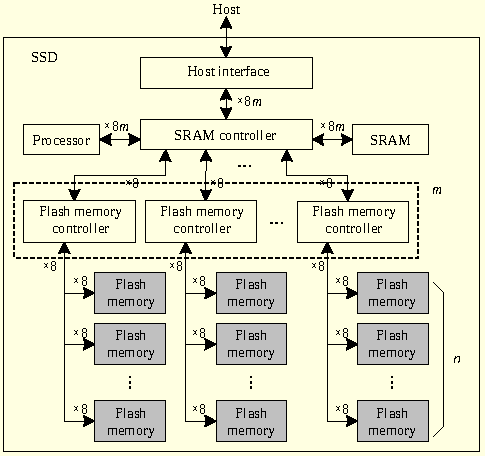
\includegraphics[width=0.6\textwidth]{figures/background/ssd_architecture.pdf}
    \caption{SSD의 $m$-channel, $n$-way 구조. 출처: Jeong 등 \cite{jeong2013}의 Fig.~4.}
    \label{fig:ssd-architecture}
\end{figure}

해당 연구진은 IOMeter를 이용해 HDD와 SSD가 처리하는 request size에 따라 throughput이 어떻게 변화하는지를 측정하였다. SSD의 읽기와 쓰기 작업 모두에서, request size가 증가할수록 throughput(단위 시간당 처리 용량)이 증가하다가, 특정 request size를 넘어가면 throughput이 증가를 멈추는 현상이 발견되었다. 이것은 request size가 커짐에 따라 SSD가 자신의 다중 채널을 병렬적으로 사용하며 채널 활용도를 최대화한 상태에 도달했기 때문이다.

해당 연구진은 SSD의 쓰기와 읽기 작업에서 이러한 throughput saturation 현상이 어떻게 달라지는지를 분석했다. SSD의 쓰기 작업에서는 순차 접근이 랜덤 접근보다 throughput이 높게 나타나는 모습을 보였다. 그런데 SSD 읽기 작업에서는 순차 접근과 랜덤 접근이 비슷한 request size에서 throughput이 포화되었고, 포화 상태의 throughput 수준도 유사하였다.

\section{Neuron Chunking}\label{sec:neuron-chunking}

LLM과 같은 모델을 휴대용 하드웨어에서 실행하는 데 있어서의 난점은, 장치의 DRAM 용량이 모델 전체를 담기에 충분하지 않은 경우가 많다는 것이다. 가중치는 플래시에 저장해두고, 중요할 것으로 예상되는 행들을 선별해 DRAM으로 가져오는 Activation Sparsification 방법론에 대한 연구가 진행되어 왔다 \cite{alizadeh2024}.

Yang 등 \cite{yang2025}은 I/O latency가 request size의 절대적인 양에 비례해서 증가할 것이라는 기존 방법론의 전제 조건에 의문을 제기하였다. 같은 양의 가중치를 읽어도, 선택한 행들이 넓은 범위에 듬성하게 분포해 있다면, throughput이 낮아질 수 있다. VLM과 같이 channel의 중요도가 균일하게 분포한 모델 가중치의 경우에서는 그러한 효과가 더 두드러질 수 있다고 저자들은 주장한다.

이에 연구진은 모델 가중치의 행들의 물리적 연속성을 반영하여 읽기 지연시간을 예측할 수 있는 chunk-based latency model을 정의하였고, 중요도-지연시간 기반 선택 방법인 Neuron Chunking을 제안하였다.

가중치 행의 수를 $N$, 선택 mask를 $M\in\{0,1\}^N$라고 하자. $M_i=1$이면 $i$번째 행을 읽는다. 토큰 수가 $H$인 입력에서 $i$번째 채널의 중요도와 mask가 보존하는 중요도를 아래와 같이 정의한다.
\[
v_i=\frac1H\sum_{t=1}^{H}|a_{t,i}|,
\qquad
I(M)=\sum_{i=0}^{N-1}v_iM_i
\]
$a_{t, i}$는 토큰 $t$의 채널 $i$번째 activation이다.

mask $M$에서 선택된 행들을 최대 연속 구간으로 분해하고 그 집합을 $\mathcal C(M)$라 하자. 길이가 $l$인 행 구간을 읽는데 걸리는 latency 비용을 $T[l]$로 정의하자. 원 논문의 chunk-based latency 모델은 다음과 같다.
\[
\widehat L_{\mathrm{table}}(M)
=\sum_{C\in\mathcal C(M)}T[|C|]
\]
연구팀은 각각의 행 구간 길이 $l$에 대해 충분한 수의 같은 크기 chunk를 읽어 처리량이 안정된 조건에서 $T[l]$를 측정하였다. $\widehat L_{\mathrm{table}}$의 정의를 이용하면 $M$에 해당하는 행들을 플래시로부터 읽어오는 데 걸리는 시간을 대략적으로 근사할 수 있다.

연구팀은 행 예산 $R$ 아래에서의 단위 추정 지연시간당 보존 중요도를 최대화하는 mask $M$을 찾고자 하는 문제를 제안하였다.
\[
\max_{\substack{M\in\{0,1\}^N\\1\le\|M\|_1\le R}}
\frac{I(M)}{\widehat L_{\mathrm{table}}(M)}.
\]
원 논문의 Greedy 알고리즘은 중요도--지연시간 비율이 높은 mask $M$을 구성하기 위해 연속 후보 구간들의 집합 $\mathcal G$를 생성한다. 각 후보 $C\in\mathcal G$에 대해
\[
U(C)=\frac{\sum_{i\in C}v_i}{T[|C|]}
\]
를 계산한다. 후보들을 점수가 높은 순서대로 검토하며, 이미 선택한 행과 겹치지 않고 잔여 예산을 넘지 않는 구간을 선택해 mask를 갱신한다.

시작 행이 $j$이고 길이가 $\ell$인 구간 후보를
\[
C_{j,\ell}=\{j,j+1,\ldots,j+\ell-1\},
\qquad 0\le j\le N-\ell
\]
로 정의하자.

행 단위로 환산한 최소·최대 후보 길이를 $\ell_{\min},\ell_{\max}$, 길이 증가 간격을 $\Delta\ell$, 시작 위치의 이동 간격 상한을 $J$라 하자. 원 논문이 후보 집합 $\mathcal G$를 구성하기 위해 고려하는 $(j,\ell)$ 쌍은 다음과 같다.
\[
\begin{aligned}
\ell&=\ell_{\min}+k\Delta\ell\le\min(\ell_{\max},N),\\
j&=m\min(\ell,J)\le N-\ell,
\end{aligned}
\qquad k,m=0,1,2,\ldots
\]
이 규칙은 $\ell>J$일 때 같은 길이의 후보 간 중첩을 허용한다. $\ell_{\max}$는 장치의 처리량 포화 지점을 기준으로 정하고, $\ell_{\min}$, $\Delta\ell$, $J$는 탐색의 세밀함과 계산량을 조절하는 매개변수로 사용한다.
